\section{Further Examples}\label{sec:examples}
\todo introductory paragraph about data structures with sharing.\\
\subsection{Concurrent Spanning Tree}
Let $\gamma$ denote a directed connected binary (DCB) graph with a finite set of vertices where each vertex is associated with at most two successors. Similarly, let $\theta$ denote an \emph{acyclic} DCB graph or a \emph{tree}. For brevity, in this section we refer to a DCB graph and an acyclic DCB graph simply as a graph and a tree, respectively. Given a graph $\gamma$, a tree $\theta$ \emph{spans} $\gamma$ if it includes all vertices of $\gamma$ with a minimal set of edges where every edge in $\theta$ is also an edge in $\gamma$. 
For instance, \fig\ref{fig:graphAndTree} depicts a DCB graph (left) and a possible spanning tree (right).
\begin{figure}
\hrule
\begin{tabular}{c c c}
	\begin{subfigure}[b]{0.3\columnwidth}
      \centering	
      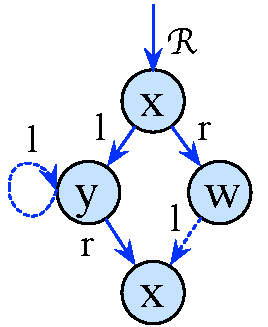
\includegraphics[scale=0.3]{sections/FurtherExamples/Images/graph.pdf}
    \caption{}
    \label{subfig:graph}
    \end{subfigure}
    &
    \begin{subfigure}[b]	{0.2\columnwidth}		
      \centering	
      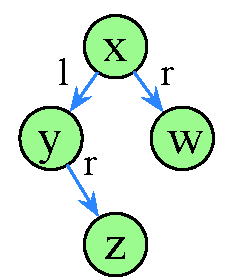
\includegraphics[scale=0.3]{sections/FurtherExamples/Images/tree.pdf}
    \caption{}
    \label{subfig:tree}
    \end{subfigure}
    &
    \begin{subfigure}[b]{0.3\columnwidth}
      \centering	
      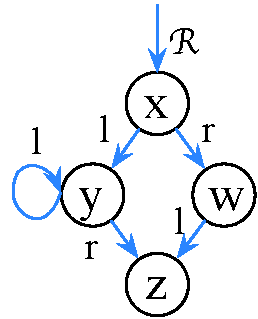
\includegraphics[scale=0.3]{sections/FurtherExamples/Images/graphWithRootEdge.pdf}
    \caption{}
    \label{subfig:graphWithRootEdge}
    \end{subfigure}
    \end{tabular}
\hrule
\caption{A directed connected binary graph (\subref{subfig:graph}), a possible spanning tree (\subref{subfig:tree}), and the same graph with the logical edge $\rootEdge$ (\subref{subfig:graphWithRootEdge}).}
\label{fig:graphAndTree}
\end{figure}
%Let $\gamma = (V, E)$ denote a connected directed binary graph where $V$ is a finite set of vertices and $E: V \rightarrow (V \uplus \{0\}) \times (V \uplus \{0\})$ is a function associating each vertex with at most two successors. Given a graph $\gamma = (V, E)$, a \emph{tree} (acyclic connected directed graph) $\theta$ is a spanning tree of $\gamma$ if it includes all vertices of $\gamma$ and every edge in $\theta$ is also an edge in $\gamma$. In other words, $\theta = (V, E')$ where $E' \subseteq E$ and $E'$ is minimal. Given a graph $\gamma = (V, E)$, we write $x \in \gamma$ for $x \in V \uplus \{0\}$.

In order to reason about graphs, we define an inductive predicate $\graph{x}{S}$ as given in \fig\ref{fig:globalCST} to describe a graph rooted at address $x$ with the finite set of vertices (addresses) $S$. It represents a spatial (in heap) graph shared amongst the threads spanning it where each node can be marked (visited) via any of its incoming edges from its predecessors. For instance, in the graph of \fig\ref{subfig:graph}, the $z$ node can be visited via the right edge of node $y$ ($y.r$) as well as the left edge of node $w$ ($w.l$). As such, in our reasoning we have \emph{marking} capabilities of the form $\markT{n}{e}$ where $n$ denotes the vertex (address) and $e$ the edge via which vertex $n$ is visited. For instance, the capabilities associated with marking of vertex $z$ in \fig\ref{subfig:graph} are $\markT{z}{y.r}$ and $\markT{z}{w.l}$. Recall from \S\ref{sec:logic} that the parameterisation of our actions are merely a notational convenience and can be substituted for their full definitions. Given a graph  at root address $x$, in order to account for the ability to mark the root vertex $x$, we introduce a logical (virtual) root edge $\rootEdge$ into $x$ as depicted in \fig\ref{subfig:graphWithRootEdge} together with its associated marking capability $\markT{x}{\rootEdge}$. The shared state contains node $x$ which can be either unmarked ($\unmarked{x}{l}{r}$) or marked ($\marked{x}$); as well as the left and right subgraphs captured recursively by the $\G{l}{S}$ and $\G{r}{S}$ predicates. Note that the two subgraphs and vertex $x$ are combined by the overlapping conjunction $\sepish$ since the graph can be cyclic and each node may be reachable via more than one path. 

Each vertex is represented as three consecutive cells in the heap tracking the mark value ($0$ or $1$) and the addresses of the left ($l$) and right ($r$) subgraphs. For brevity, we write $\cell{x}{m, l, r}$ for $\cell{x}{m} * \cell{x+1}{l} * \cell{x+2}{r}$. Moreover, in order to increase readability we write $x.m$, $x.l$ and $x.r$ for $x$, $x+1$ and $x+2$, respectively. When vertex $x$ is in the unmarked state, the mark value corresponds to $0$ ($\cell{x.m}{0}$) and the left and right pointers ($\cell{x.l}{l} * \cell{x.r}{r}$) as well as the capability to mark them ($\markT{l}{x.l} * \markT{r}{x.r}$ reside in the shared state. In the marked state the mark value is $1$ ($\cell{x.m}{1}$) and the resources associated with the left and right subgraphs (pointers and capabilities) have been claimed by the marking thread. 

The interference associated with the graph is described as the union of interferences pertaining to the vertices of the graph ($S$). For each vertex $n \in S$, the only permitted action is that of marking $n$ which can be carried out by any of the marking capabilities associated with node $n$ ($\markT{n}{-}$). Note that the anonymous quantification $-$ is yet another notational shorthand and can be substituted for the following more verbose definition.
%%
%\[
%I(n) \eqdef \bigcup\limits_{p \in S} \left( \bigcup\limits_{e \in \{p.l, p.r, \rootEdge\}} \markT{n}{e} : \exsts{l, r} \unmarked{n}{l}{r} \swap \marked{n} \right)
%\]
%%
%
\[
I(n) \eqdef \bigcup\limits_{e \in \textsf{Loc}} \markT{n}{e} : \exsts{l, r} \unmarked{n}{l}{r} \swap \marked{n} 
\]
%
%
\begin{figure}
%
\hrule
\[
\begin{array}{r @{\hspace*{2pt}} l}
	\graph{x}{S} \eqdef & \markT{x}{\rootEdge} * \shared{\G{x}{S}}{\bigcup\limits_{n \in S}I(n)}\\
%	
	\G{x}{S} \eqdef & (x = \nil \land \emp) \lor x \in S \land \exsts{l, r}\\
	& \left( \unmarked{x}{l}{r} \lor \marked{x}\right) \sepish \G{l}{S} \sepish \G{r}{S}\\
%
	\unmarked{x}{l}{r} \eqdef & \cell{x}{0, l, r} * \markT{l}{x.l} * \markT{r}{x.r}\\
%	
	\marked{x} \eqdef & \cell{x}{1}\\
%
	I(n) \eqdef & \left\{ \markT{n}{-}: \exsts{l, r} \unmarked{n}{l}{r} \swap \marked{n}\right\}\\
%
%	\tree{x}{S} \eqdef & \markT{x}{\rootEdge} * \shared{\G{x}{S}}{\bigcup\limits_{n \in S}I(n)}\\
\end{array}
\]
%
\hrule
\caption{Global specification of the graph predicate.}
\label{fig:globalCST}
\end{figure}
%
%
\fig\ref{fig:conSpanningTree} shows an in place concurrent algorithm for calculating a spanning tree of a graph. It proceeds by recursively marking the vertices to keep track of those already visited; the return value b records the outcome of marking with b=$true$ when the top node $x$ is unmarked (not visited yet) and b=$false$ otherwise. Assuming that the root vertex $x$ is unmarked initially, the algorithm continues by first marking $x$ and subsequently spanning the left and right subgraphs concurrently. When the top node of the left subgraph is already marked (!b1), the edge from $x$ into it is replaced by a null pointer. This corresponds to the case where the node has already been visited by another thread and is thus reachable from the root; \emph{mutatis mutandis} for the right subgraph.
%
\begin{figure}
%
\hrule
\[
\begin{array}{r @{\hspace*{2pt}} l}
	\g{x}{S} \eqdef & (x = \nil \land \emp) \lor x \in S \land \exsts{l, r}\\
	& \shared{\unmarked{x}{l}{r} \lor \marked{x}}{I(x)} * \g{l}{S} * \g{r}{S}\\
	
	\tr{x}{S} \eqdef & (x = \nil \land \emp) \lor \\
	& x \in S \land \exsts{l, r}\exsts{l' \in \{l, \nil\}} \exsts{r' \in \{r, \nil\}}\\
	&  \shared{\marked{x}}{I(x)} * \markT{l}{x.l} * \cell{x.l}{l'} * \tr{l'}{S} * \\
	&  \markT{r}{x.r} * \cell{x.r}{r'} *\tr{r'}{S}
\end{array}
\]
\hrule
\label{fig:localCST}
\caption{Local specification of the graph predicate.}
\end{figure}
%
The $\graph{x}{S}$ predicate defined in \fig\ref{fig:globalCST} is a \emph{global} account of the graph in that it captures all vertices and the interference associated with them. However, our spanning tree algorithm operates \emph{locally} as it is called upon recursively for each node. That is, for each $\texttt{span}(n)$ call (where $n \in S$), the footprint of the call is limited to node $n$. Moreover, in order to reason about the concurrent recursive calls $\texttt{span(x.l) || span(x.r)}$, we need to \emph{split} the state into two $*$-composed states prior to the calls, pass each constituent state onto the relevant thread and combine the resulting states by $*$ composition through an application of the \textsc{Par} rule. We thus provide a \emph{local} specification of the graph, $\g{x}{S}$ as defined in \fig\ref{fig:localCST} such that for all $S in \pset{\textsf{Loc}}$ and $n, e \in S$  \\

\todo explain the $\g{x}{S}$ and $\tr{x}{S}$ predicates. 
%
\[
	\left\{
	\begin{array}{@{} l @{}}
		\markT{n}{p} * \\
		\g{n}{S}
	\end{array}
	\right\}  
%	
	b\texttt{:= span(}n\texttt{)} 
%
	\left\{
	\begin{array}{@{} l @{}}
		\markT{n}{p} * 
		\left(
		\begin{array}{@{} l @{}}
			b \land \tr{n}{S} \lor\\
			\neg b \land \tr{\nil}{S}
		\end{array}
		\right)
	\end{array}
	\right\}
\]
%


We now demonstrate how to obtain the local specification $\g{x}{S}$ from the global specification of \fig\ref{fig:globalCST}. 
When expanding the definition of $\G{x}{S}$, there are two cases to consider depending on whether or not $x = \nil$. In what follows we only consider the case where $x \not= \nil$ since the derivation in the case of $x = \nil$ is trivial.
%
\[
\begin{array}{@{} c @{} l @{}}
	&\shared{\G{x}{S}}{\bigcup\limits_{n \in S} I(n)}  \\
	
	\stackrel{(\textsf{G}\ \defin)}{\implies} & \shared{\exsts{l, r} (\unmarked{x}{l}{r} \lor \marked{x}) \sepish \G{l}{S} \sepish \G{r}{S}}{\bigcup\limits_{n \in S} I(n)} \\
	
	\implies &   \exsts{l, r}  \shared{(\unmarked{x}{l}{r} \lor \marked{x}) \sepish \G{l}{S} \sepish \G{r}{S}}{\bigcup\limits_{n \in S} I(n)} \\
	
	\stackrel{(\textsc{Copy})}{\implies} &
	\exsts{l, r}  
	\shared{(\unmarked{x}{l}{r} \lor \marked{x})  \sepish \G{l}{S} \sepish \G{r}{S}}{\bigcup\limits_{n \in S} I(n)} \\
	& * \shared{(\unmarked{x}{l}{r} \lor \marked{x}) \sepish \G{l}{S} \sepish \G{r}{S}}{\bigcup\limits_{n \in S} I(n)} \\
	& * \shared{(\unmarked{x}{l}{r} \lor \marked{x})  \sepish \G{l}{S} \sepish \G{r}{S}}{\bigcup\limits_{n \in S} I(n)} \\
	
	
	\stackrel{(\textsc{Forget})}{\implies} &
	\exsts{l, r}  
	\shared{\unmarked{x}{l}{r} \lor \marked{x}  }{\bigcup\limits_{n \in S} I(n)} \\
	& * \shared{\G{l}{S}}{\bigcup\limits_{n \in S} I(n)} * \shared{\G{r}{S}}{\bigcup\limits_{n \in S} I(n)} \\
	
	
	
	\stackrel{(?)}{\semimplies} &
	\exsts{l, r}  
	\shared{\unmarked{x}{l}{r} \lor \marked{x}}{\bigcup\limits_{n \in S} I(n)} * \g{l}{S} * \g{r}{S}\\
	
	
	\stackrel{(\textsc{Shift})}{\semimplies} &
	\exsts{l, r}  
	\shared{\unmarked{x}{l}{r} \lor \marked{x} }{I(x)} * \g{l}{S} * \g{r}{S}\\
	
	
	\iffdef & \g{x}{S}
	
\end{array}
\]
%
%
\begin{figure}
\hrule
\begin{lstlisting}
 //$\comment\{\graph{x}{S}\}$
 //$\comment\{\markT{x}{\rootEdge} * \shared{\G{x}{S}}{\bigcup\limits_{n \in S} I(n)}\}$
 //$\comment\{\markT{x}{\rootEdge} * \g{x}{S}\}$
 b:= span(x) {
   //$\comment\{\markT{x}{\rootEdge} * \shared{\exsts{l, r} \unmarked{x}{l}{r} * \g{l}{S} * \g{r}{S}  \lor \marked{x}}{I(x)} \}$
   res:= <CAS(x.m, 0, 1)>;
   //$\comment\left\{\begin{array}{l}\markT{x}{\rootEdge} * \shared{\marked{x}}{I(x)} *\\ (\neg\texttt{res}\land\emp) \lor\\  \left(\begin{array}{l}\texttt{res}\land\exsts{l, r} \cell{x.l}{l} * \cell{x}{r} *\\ \markT{l}{x.l} * \g{l}{S} * \markT{r}{x.r} * \g{r}{S} \end{array}\right)\end{array}\right\}$
   if (res) then { 
   //$\comment\left\{\begin{array}{l} \texttt{res} \land \exsts{l, r} \markT{x}{\rootEdge} * \shared{\marked{x}}{I(x)} * \cell{x.l}{l} * \cell{x}{r} *\\\markT{l}{x.l} * \g{l}{S} * \markT{r}{x.r} * \g{r}{S} \end{array}\right\}$
     //$\comment\left\{\markT{l}{x.l} * \g{l}{S} * \markT{r}{x.r} * \g{r}{S}  \right\}$   
     b1:= span(x.l) || b2:= span(x.r)
     //$\comment\left\{\begin{array}{l}\markT{l}{x.l} * \left( (\texttt{b1} \land \tr{l}{S}) \lor (\neg\texttt{b1} \land \tr{\nil}{S})\right) *\\ \markT{r}{x.r} * \left( (\texttt{b2} \land \tr{r}{S}) \lor (\neg\texttt{b2} \land \tr{\nil}{S})\right)  \end{array}\right\}$   
   //$\comment\left\{\begin{array}{l}  \texttt{res} \land \exsts{l, r} \markT{x}{\rootEdge} * \shared{\marked{x}}{I(x)} * \cell{x.l}{l} * \cell{x}{r} *\\ \markT{l}{x.l} * \left( (\texttt{b1} \land \tr{l}{S}) \lor (\neg\texttt{b1} \land \tr{\nil}{S})\right) *\\ \markT{r}{x.r} * \left( (\texttt{b2} \land \tr{r}{S}) \lor (\neg\texttt{b2} \land \tr{\nil}{S})\right)   \end{array}\right\}$  
     if (!b1) then 
       x.l:= null
     if (!b2) then 
       x.r:= null
   //$\comment\left\{\begin{array}{l}  \texttt{res} \land \exsts{l, r} \markT{x}{\rootEdge} * \shared{\marked{x}}{I(x)} * \\ \exsts{l' \in \{l, \nil\}} \markT{l}{x.l} * \cell{x.l}{l'} * \tr{l'}{S} *\\ \exsts{r' \in \{r, \nil\}} \markT{r}{x.r} * \cell{x}{r'} * \tr{r'}{S} \end{array}\right\}$      
   //$\comment\{\texttt{res} \land \markT{x}{\rootEdge} *  \tr{x}{S}\}$      
   }		
   //$\comment\{(\texttt{res} \land \markT{x}{\rootEdge} * \tr{x}{S}) \lor (\neg \texttt{res} \land \markT{x}{\rootEdge} * \shared{\marked{x}}{I(x)}) \}$   
   //$\comment\{\markT{x}{\rootEdge} *  (\texttt{res} \land \tr{x}{S}) \lor (\neg \texttt{res} \land \tr{\nil}{S}) \}$      
   return res
 }
 //$\comment\{\markT{x}{\rootEdge} *  (\texttt{b} \land \tr{x}{S}) \lor (\neg \texttt{b} \land \tr{\nil}{S}) \}$      
\end{lstlisting}
\hrule\vspace*{5pt}
\caption{Concurrent Spanning Tree Implementation}
\label{fig:conSpanningTree}
\end{figure}
%

\todo Briefly touch the proof of \fig\ref{fig:conSpanningTree}.

\subsection{Set Example}
\azaleaComment{ We don't have enough space to cover this here, it will have to go into the tech report. We should mention it here though.}